\documentclass[10pt,twocolumn,letterpaper]{article}

\usepackage{cvpr}
\usepackage{times}
\usepackage{epsfig}
\usepackage{graphicx}
\usepackage{amsmath}
\usepackage{amssymb}
\usepackage{dsfont}
\usepackage{tablefootnote}
\usepackage{multirow}
\usepackage{subcaption}
% \usepackage{caption}
\usepackage[ruled]{algorithm2e}
% Include other packages here, before hyperref.

% If you comment hyperref and then uncomment it, you should delete
% egpaper.aux before re-running latex.  (Or just hit 'q' on the first latex
% run, let it finish, and you should be clear).
\usepackage[pagebackref=true,breaklinks=true,letterpaper=true,colorlinks,bookmarks=false]{hyperref}

% \cvprfinalcopy % *** Uncomment this line for the final submission
\DeclareCaptionFont{9pt}{\fontsize{9pt}{10pt}\selectfont}
\captionsetup[figure]{textfont=9pt}
\captionsetup[table]{textfont=9pt}
\def\cvprPaperID{3035} % *** Enter the CVPR Paper ID here
\def\httilde{\mbox{\tt\raisebox{-.5ex}{\symbol{126}}}}

% Pages are numbered in submission mode, and unnumbered in camera-ready
\ifcvprfinal\pagestyle{empty}\fi

\newcommand{\norm}[1]{\left \lVert #1 \right \rVert_{F}^2}
 \newcommand{\normtwo}[1]{\left \lVert #1 \right \rVert_2^2}
\DeclareMathOperator*{\argmax}{arg\,max}
\DeclareMathOperator*{\argmin}{arg\,min}
\DeclareMathOperator*{\minimize}{min}

\begin{document}

%%%%%%%%% TITLE
\title{Semi-supervised Zero-Shot Learning by a Clustering-based Approach}

\author{CVPR Submission 3035}

\maketitle
%\thispagestyle{empty}

%%%%%%%%% ABSTRACT
\begin{abstract}
In some of object recognition problems, labeled data may not be available for all categories. Zero-shot learning utilizes auxiliary information (also called class signatures) describing all categories in order to find a classifier that can also recognize samples
from categories with no labeled instance.
In this paper, we propose a novel semi-supervised zero-shot learning method that works on a representation space corresponding to abstract deep visual features. We use the idea that the rich deep visual features provide a representation space in which samples of each class are usually condensed in a cluster. We seek a transformation on signatures to map them onto the visual features, such that the mapped signatures of the seen classes are close to labeled samples of the corresponding classes and unlabeled data are also close to the mapped signatures of one of the unseen classes.
The effectiveness of the proposed method is demonstrated through extensive experiments on four public benchmarks and we show that our method improves the state-of-the-art prediction accuracies.

\end{abstract}



\section{Introduction}
Zero-shot learning \cite{bengio08,hinton09,lampert09,farhadi09} is an extension to the conventional supervised learning scenario
that releases the assumption of having ample labeled instances for all categories. It addresses the
recognition problem in which no labeled instance is available for some classes but
some sort of description that is called \textit{class signature} is available for all categories.
Example of class signatures include human-annotated discriminative attributes or textual description of the categories.
The problem addressed by zero-shot learning rises naturally in practice wherever it is not feasible to acquire abundant labeled instances for
 all categories (e.g., fine-grained classification problems).
To describe the task more precisely, in the training phase, labeled instances for some categories called seen classes are provided
while for other categories, called unseen ones, there is no labeled instance available.
In the test phase, unlabeled instances should be classified into seen or unseen categories.
 In this work, we focus on the most popular version of zero-shot recognition in which test instances belong only to unseen categories.
 %In this setting, zero-shot learning mitigates the problem of acquiring labeled instances, which can be hard for a novel, rare or fine-grained categories.
 \begin{figure*}[t]
 \begin{center}
 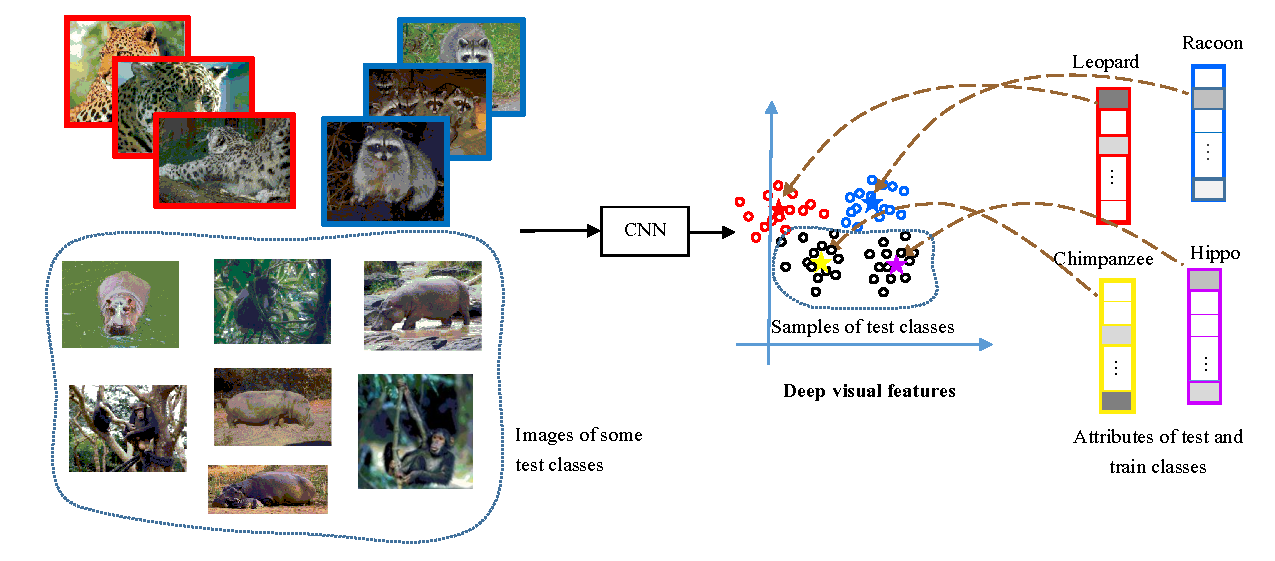
\includegraphics[width=2\columnwidth]{FigOverview.pdf}%{overview.pdf}
 %\caption{In our model, we map class signatures close to all instances of the class for seen classes and close to instances in a cluster for unseen ones.
%Here, clusters are shown by ellipses and class signatures mapped to the center of these clusters are depicted by stars.}
\caption{The proposed method maps attribute vectors of classes to the space of deep visual features such that the mapped attribute vectors are good representatives for the samples of the corresponding classes. The mapped attributes are depicted by stars.}
 \label{fig:overview}
 \end{center}
 \end{figure*}
Most existing methods for zero-shot learning focus on using labeled instances (i.e. images) to learn a compatibility function indicating how similar an instance is
to each label embedding obtained from class signatures~\cite{Akata2015,emb15,sse}. Each instance will then be labeled with the category having the most compatible signature.
 On the other hand, recent advances in deep neural networks provide rich visual features with high discrimination capability~\cite{vgg}.
We found out through experiments that the space of deep visual features is a rich space in which instances of different categories usually form natural clusters.
Nonetheless, little attention has been paid to exploiting this property of deep visual features in the context of zero-shot learning.

 %In the previous works, most concentration has been on finding embeddings for visual features and little effort has been made to exploit unsupervised information in images domain.

In this paper, we propose a semi-supervised zero-shot
learning method called \textit{Joint Embedding and Clustering} (JEaC) that uses both labeled instances of seen
classes and unlabeled instances of unseen classes to find a
more proper representation of class signatures in the space of deep visual features. In this method, a linear transformation
is learned to map the class signatures to the space of
abstract visual features and jointly assignments of unlabeled
samples to unseen classes are found (Figure~\ref{fig:overview}).
The linear mapping is learned so that the mapped signature of each seen class tends to be representative
for samples of the corresponding class and simultaneously
assignments of unlabeled samples to unseen classes are leaned such that the mapped signature of each unseen class
 also tends to be representative of assigned samples to that class.
 Using unlabeled samples from unseen classes, we can substantially mitigate
the \textit{domain shift problem} introduced in \cite{eccv14} that impairs the zero-shot recognition performance.
We also propose a simpler method called \textit{Independent Embedding and Clustering} (IEaC) in which label assignment and class embedding in the image space are not learned jointly. Instead,
after finding the mapping according to just instances of seen
classes, a clustering algorithm is used to assign labels to instances
of unseen classes.

%To show the capability of our proposed method that jointly learns the linear transformation on class signatures and label assignments to unlabeled data, we also propose simpler methods that do not use these ideas altogether. Indeed, we also propose two simpler methods that only optimizes one of these two objectives and also a method that considers both of these objectives but does not simultaneously optimizes them. Indeed, after finding the mapping, it uses a clustering algorithm to assign samples of unseen classes to those classes. A semi-supervised clustering algorithm is proposed for this purpose to leverage labels available for seen classes to obtain more accurate cluster assignments.
 %A semi-supervised clustering algorithm is proposed for this purpose to leverage labeled instances available for seen classes to obtain more accurate cluster assignments.
We present experimental results on four popular zero-shot classification benchmarks
 and see that the proposed method outperforms state-of-the-art methods on these datasets.


%___________________________________________________________________________________________________________________________________________________________
%______________________________________Related Work_________________________________________________________
\section{Related Work} \label{related}
% Most existing methods for zero-shot object recognition can be described as finding a compatibility function scoring how
% similar an image and a description are.
% We can consider three tasks for these methods:
%   1) Find (or use the existing) embeddings for class labels in a semantic space.
%   2) Map images into that semantic space.
%   3) Classify images in the semantic space based on the compatibility of the mapped image and the embedded labels in this space (usually using a nearest neighbor classifier or label propagation).
% Learning of these three steps may be done independently or jointly.

A notable body of work in zero-shot recognition belongs to attribute prediction from images \cite{lampert09,topicmodel,ajoint11,unified13,suzuki14}.
In these methods, the semantic label embeddings are considered to be externally provided attributes. Thus, label embeddings are already available
 and the task is just to map images to the semantic space, i.e. predicting attributes for the images.
Early methods, like \cite{lampert09} do not consider dependency of attributes and train binary attribute classifiers.
Probabilistic graphical models have been utilized to model and/or learn correlations among different attributes \cite{topicmodel,unified13}
 to improve the prediction.
In \cite{jayaraman14}, a random forest approach has been employed that accounts for unreliability in attribute predictions for final class assignment.
In \cite{akata13}, a max-margin objective function
% similar to the structured SVM
is defined for attribute-based image classification.
% When the label embeddings are fixed, it can be used for zero-shot recognition.

More recent works often exploit bilinear models \cite{Yu2013,devise,convex,sse,emb15,semi15}.
 Several objective functions have been proposed for learning such bilinear models.
In \cite{emb15}, the sum of the squared error on the label prediction is used and clever regularization
 terms that compensate undesirable characteristics of this cost function are also utilized.
% This method can be seen as learning a mapping that transforms description of each class to a linear classifier for that class.
In \cite{li15max,semi15}, a max margin objective function for learning the bilinear mapping is used.
 These two methods learn labels for test instances simultaneously and so they differ from almost all of other existing methods in this way.
 They provide the possibility of
leveraging unsupervised information available in test images. In \cite{semi15},
the distribution of unlabeled instances is entered through using a Laplacian regularization term that penalizes similar objects assigned to different classes.

Designing label embeddings in the multi-class classification problem
% that can be considered as a general framework for multi-class classification
is another line of research that can also be used in zero-shot recognition.
 % For a label embedding to be helpful in classification tasks,
 % it should exhibit two properties \cite{Yu2013}: 1) category-separability and 2) learnability.
 In \cite{Yu2013}, an objective function is proposed to derive such label embeddings based on information about similarities among categories.
A relatively popular embedding for labels is to describe unseen categories as how similar they are to the seen ones.
% One way to use this embedding is creating classifiers for unseen categories by linear combination of
% classifiers for seen categories using similarity scores as mixing weights.
In \cite{convex}, the outputs from the softmax layer of a CNN trained on seen categories are used to score similarity between test instances and seen classes.
Using these outputs as weights, images are represented in the semantic space as a convex combination of seen class labels embedding.
In \cite{sse}, a histogram showing seen class proportions is used for label embedding and then a max margin framework is defined to embed images in this space.
This work is further extended in \cite{agnostic} and a supervised dictionary learning formulation is presented to jointly learn embedding for images and labels.
%
 The idea of combining already available classifiers to create new ones for unseen categories is also used in \cite{Synthesized}
 but rather than using seen categories as basis, they define a set of (possibly smaller) \textit{phantom} classes and learn base classifiers on them.


 Although most of the works on zero-shot recognition consider attributes as auxiliary information,
textual descriptions or name of the categories can also be utilized as class signatures.
 \cite{devise} introduce a bilinear model to find the compatibility score of deep visual features and Word2vec \cite{word2vec} representation of class names.
\cite{ba2015} proposes nonlinear mappings modeled by neural networks on the image and the text inputs to find their compatibility.
\cite{mohamed13} presents an objective function to predict classifier parameters from textual descriptions.
 In \cite{Akata2015}, some different label embeddings and also a combination of these embeddings have been considered along with a bilinear
 compatibility function.
  In \cite{Xian2016}, this work is extended further to model nonlinear compatibility
 functions that can be expressed as a mixture of bilinear models.
   % Intuitively, different linear models will use different aspects of images to measure the compatibility and the proper aspect is selected automatically for every test image.s
  % In \cite{Qiao2016}, a modification of \cite{emb15} is presented as for use with textual auxiliary information by decomposing the bilinear mapping.
In \cite{Fu2016}, a set of vocabulary much larger than just seen and unseen class names is used and mapping from images to word embeddings is learned
by  maximizing the margin with respect to all words in the vocabulary;
 this framework can be used in zero-shot and also supervised and open set learning problems. In \cite{ziad16} a tensor factorization approach is used
 to predict attribute vectors for unseen categories using word embedding of their names, solving the problems in which no
 attribute vector is provided for unseen categories (e.g. open set learning problem) by creating attribute vectors and then classifying using
 Direct Attribute Prediction \cite{lampert09}.
 In  \cite{Akata2016}, authors propose to use multiple auxiliary information and also
 semantic part annotations in the image domain to compensate for weaker supervision in textual data.
%The nature of zero-shot learning problem in which usually only one document exists for each category has hindered using more sophisticated models for text embedding.
Convolutional and recurrent neural networks have also been used for text embedding in \cite{Akata2016rnn}.

The most related methods to ours are \cite{li15max,Kodirov2015,semi15}
 that are semi-supervised zero-shot learning methods.
Here, we briefly specify the differences between these methods and ours.
 First, we use abstract visual features obtained by deep learning as the semantic space as opposed to \cite{li15max,semi15}.
 These two methods learn a max margin classifier on the image space classifying both seen and unseen
instances while we propose a clustering-based approach in the semantic space of deep visual features that uses a ridge regression to map signatures to this semantic space. Our approach results in a much simpler optimization problem to solve.
% Since samples of different classes are usually condensed in distinct regions of the deep visual representation space,
%  our proposed optimization problem is based on clustering of data in this space and we try to map the class
% signatures on the centroid of the corresponding samples.
 We also explicitly account for domain shift problem in our objective function and thus achieve better results compared to these methods.
%
There are major differences between our work and ~\cite{Kodirov2015} using a dictionary learning scheme
in which coding coefficients are considered to be label embeddings (attribute vectors) and a sparse coding objective is used to map images into this representation space.
Most importantly, in our method, labels of unseen instances are jointly learned
with the mapping of the signatures to the semantic space while in \cite{Kodirov2015}
the label prediction is accomplished using the nearest neighbor or the label propagation on embeddings of images.
Moreover, we do not need to learn embedding of test instances in the semantic space as opposed to \cite{Kodirov2015},
alternatively we learn just the representation of class signatures in the visual domain.

\section{Proposed Method} \label{proposed}
In this section, we introduce two zero-shot learning methods that use deep visual features as the semantic space and learn
a mapping from class signatures to this semantic space. % and find labels for instances belonging to unseen classes.
 First, we propose Independent Embedding and Clustering (IEaC) as a simple and efficient semi-supervised zero-shot learning method.
Then, we further extend our method to jointly learn the embedding of signatures and class assignments of unlabeled samples.
We call this method Joint Embedding and Clustering (JEaC). We formulate an optimization problem for JEaC and
 present an iterative method to solve it.
IEaC is used to find a proper starting point for this optimization procedure
 (i.e. labels found by IEaC for instances of unseen classes are considered as initial label assignment to these instances).
\subsection{Notation}
Let $X, \mathbf{x}$, and $x$ denote matrices, column vectors, and scalars respectively. $\norm{X}$ shows the squared Frobenius norm of a matrix and
$X_{(i)}$ denotes its $i$th column. $\mathbf{1}_k$ denotes a column vector whose $k$-th element is one and other elements are zero.
Suppose there are $n_s$ seen categories and $n_u$ unseen categories. For each category $y$,
auxiliary information $a_y \in \mathbb{R}^r$ is available. We assume that labels $\{1, \ldots, n_s \}$ correspond to seen categories.

Let $X_s \in \mathbb{R}^{d \times N_s}$ and $X_u \in \mathbb{R}^{d \times N_u}$
denote matrices whose columns are seen and unseen images respectively where $d$ is the dimension of image features and $N_s$ (or $N_u$) shows the whole number of the images in the seen (or unseen) classes.
$S_s = [a_1, \ldots, a_{n_s}]$ presents the matrix of signatures for seen classes and $S_u$ is defined similarly for unseen classes.
$Z_s = [ \mathbf{z}_1, \ldots, \mathbf{z}_{N_s} ]$
contains labels of training data in the one-hot encoding format. $\mathbf{r}_n$ also denotes the label assigned to the $n$-th instance by our algorithm in the one-hot coding format.

\subsection{Independent Embedding and Clustering} \label{clustering}
Our first method can be roughly summarized in three steps:
\begin{enumerate}
  \item
   Using data from seen classes, we learn a linear mapping from attribute vectors to the semantic space.
  \item We find a data clustering using our proposed semi-supervised clustering algorithm.
  \item For each cluster, we find the label whose mapped signature in the semantic visual space is the nearest one to the center of that cluster
   and assign the corresponding label to all of its instances.
\end{enumerate}
We use a simple ridge regression to map class signatures to deep visual features.
 We intend to a mapping such that each mapped (seen) class signature is close to the samples of that class in this space in average.
The linear mapping is found using the following optimization problem:
\begin{equation} \label{eq:mapping}
  W^* = \argmin_W \norm{X_s - W Y_s} + \gamma \norm{W},
\end{equation}
where columns of $ Y_s \in \mathbb{R}^{r \times n_s} $ are the class signatures of the samples lied in the columns of $X_s$ (i.e. $Y_s=S_sL$ where columns of $L$ contain the one-of-$n_s$ encoding of the labels for instances of seen classes).
This optimization problem is known to have the following closed form solution:
\begin{equation} \label{eq:dic}
  W = X_s Y_s^T (Y_s Y_s^T + \gamma I)^{-1}.
\end{equation}
The parameter $\gamma$ is determined through cross validation as we will describe in the Experiments section.

Here, we intend to find labels for the instances belonging to unseen classes. To this end, we find a clustering of instances
 in the space of deep visual features and then assign a label to each cluster according to the distance between the center of that cluster
 and the mapped signatures of unseen classes.
The label whose mapped signature is the closest one to the cluster center is selected to be assigned to all instances in the cluster.
More precisely, let $\boldsymbol{\mu}_k$ be the center of the $k$-th cluster and $c(\mathbf{x}_n)$ denote the cluster number to which $\mathbf{x}_n$ is assigned.
The label assigned to $\mathbf{x}_n$ in our method would be:
\begin{equation} \label{eq:label_assign}
  \argmin_{i=n_s + 1,\ldots, n_u + n_s} \normtwo{ W(Y_s)_{(i)} - \boldsymbol{\mu}_{c(\mathbf{x}_n)} }.
\end{equation}

To find a better clustering of instances belonging to unseen classes,
 we can also incorporate labeled instances of seen classes.
  The clustering problem over unseen instances with which we encounter here is different from the conventional semi-supervised learning problem \cite{chapel06}.
Here, all labeled data are from seen classes and there is no labeled sample for unseen classes that is due to the special characteristic of zero-shot
 learning problem. Therefore, we propose a semi-supervised clustering method which can be seen as an extension of k-means that is properly
 adapted for zero-shot learning problem.
 We try to find a clustering such that labeled instances tend to be assigned to the corresponding classes
  and all instances tend to be close to the center of the clusters to which they are assigned:
\begin{equation} \label{eq:simple}
\minimize_{R, \boldsymbol{\mu}_1, \ldots, \boldsymbol{\mu}_k }  \sum_{n,k} r_{nk} \lVert \mathbf{x}_n - {\mu}_k \rVert_2^2 +
 \beta \sum_{n=1}^{N_s} \mathds{1}(\mathbf{r}_n \neq \mathbf{z}_n),
\end{equation}
where $\boldsymbol{\mu_i}$s are cluster centers and $R = [\mathbf{r}_1, \ldots, \mathbf{r}_{N_s + N_u } ]$ contains cluster assignments
 of all instances in one-hot encoding format.
The objective function is similar to that of the k-means clustering algorithm but for each labeled instance
 there is a penalty of $\beta$ if the assigned cluster number is different from its label. Thus, this objective function encourages
the first $n_s$ clusters be corresponding to the seen classes.
%This is intuitively plausible, on one hand all data is being used in the clustering and on the other ????????

Parameters $\beta$ and $k$ can be determined via cross validation. However, in our experiments, we found out
the model is not very sensitive to them so we fix $\beta=1$
when data have been normalized. \textcolor{red}{ Moreover, we set $k =  (n_s + 2n_u)$ which
can allow more than one cluster per class for unseen categories. This, to some extent, copes with diversity of instances in a class.}

To solve the optimization problem in Eq.~\ref{eq:simple}, we use an iterative procedure (similar to k-meams) shown in Algorithm~\ref{alg:ieac}. In each iteration, $\mathbf{\mu}_i$s are updated as:
\begin{equation} \label{eq:updata_mu}
  \mu_i = \frac{\sum_{n=1}^{N_s + N_u}  \mathds{1}(r_{ni}=1)\mathbf{x}_n}{\sum_{n=1}^{N_s+N_u}\mathds{1}(r_{ni}=1)},
\end{equation}
and instances of unseen classes are assigned to the nearest cluster to them.

To initialize $\boldsymbol{\mu}_i$'s, for clusters corresponding to seen classes the centers are set as the mean of instances of those classes. Centers of other
clusters are initialized using k-means++ \cite{kmeanspp} on unlabeled instances.

% Finally, to assign labels to test instances, we use the mapping $W$ from Eq.\eqref{eq:dic} to
% map class signatures to visual features, creating a set of \textit{class representatives}
%  in the visual feature space. We then assign to all instances of a cluster the class label whose representative is
%   the nearest to the center of that cluster.
%We argue that the this method of assigning labels to clusters rather than individual instances can mitigate the domain shift problem in zero-shot learning.

% We argue that this learning scheme can mitigate domain shift problem  between seen and unseen categories and thus achieve higher classification accuracy.

%This is specifically favorable in our setting where we want to use this mapping to classify cluster centers that also approximate \textit{average} of class instances.

%Because all members of each cluster is assumed to share the same label. To overcome this bottleneck, in the next section we present a joint frame work to learn cluster assignments jointly with the mapping.
A key distinction between the clustering-based method presented here and other existing methods lies in the nature of the compatibility function.
 The compatibility function in other works is usually a similarity measure between each instance and class description. This measure is found independently for different instances.
 Here, the compatibility function relies strongly on the distribution of instances in the semantic space and the compatibility of a label for an instance is found
according to the similarity of the cluster center to which this instance is assigned and the mapped signature of that label.
Therefore, by considering the distribution of data samples (via clustering)
in designing the compatibility function, we can reach a more reliable measure.
% This compatibility function can be plugged in every other method in this way that after final predictions are made by the method,
% a clustering algorithm is ran on data and then we assign an identical label to all cluster
% members by majority voting on those predictions.
 % We found through experiment that this extra step will improve performance of many existing methods.

Although the above method outperforms the state-of-the-art methods on most zero-shot recognition benchmarks, it uses only instances of the seen classes to find the linear transformation from class signatures to the visual feature space and thus the proposed method may suffer from the domain shift problem introduced in \cite{eccv14}.
To overcome the domain shift problem more substantially, in the next subsection, we propose an optimization problem for finding the linear transformation from class signatures to the visual feature space that uses instances of both seen and unseen classes.

\subsection{Joint Embedding and Clustering}
\label{joint}
%In the method we proposed earlier, once the the points are assigned to a cluster, they all will inevitably share an identical label. This can limit the performance of the method. One example arises for cluster \textit{outliers} that are distant from center of their cluster but lie nearby a landmark. This instances most probably belong to the class of nearby landmark but will be labeled same as their cluster center.
In this section,
 we present an optimization problem for jointly learning a linear transformation
from class signatures to the visual feature space and assigning of unlabeled instances to unseen classes.
Accordingly, we seek a linear transformation (and simultaneously cluster assignments of unseen data)
such that the mapped signatures are good representatives of the assigned instances to the corresponding classes.
 We then present an iterative procedure to solve the proposed optimization problem.

The objective function of JEaC is formulated as follows:
 \begin{align} \label{eq:main}
   \minimize_{R,W} \norm{X_s - W Y_s}  &+ \lambda \norm{X_u - W S_u R^T } + \gamma \norm{W}, \\
   \text{s. t.} \quad & R \in \{0,1\}^{N_u \times n_u}. \nonumber
 \end{align}
where $R$ shows the cluster assignment of unlabeled instances in one-hot encoding format. The first term in the above optimization problem is identical to Eq.\eqref{eq:mapping} and the second one incorporates unlabeled data for learning the mapping $W$. Therefore, we seek class assignments for instances of unseen classes and simultaneously learn a mapping on the class signatures such that the mapped signatures provide good representatives for instances of both the seen and unseen classes. By enforcing
 the signatures of unseen classes to be mapped close to a set of test instances, the second term helps us to confront the domain shift problem.
More precisely, in the above problem, for the seen classes, the sum of the squared distances of instances from the
 mapped signature of the corresponding class is minimized. For instances of unseen classes,
 the mapping and class assignment are jointly learned to minimize such term (i.e. sum of their squared distances from representation of the class they are assigned to).
  The second term in Eq.~\ref{eq:main} can be essentially considered as a clustering objective with two
  additional advantages. First, the number of clusters is no longer a parameter and is determined by the number of unseen classes.
   Second, the cluster centers are set to be the mapped signatures of the test classes and thus we can learn mapping $W$ and class assignments $R$ jointly.

\subsubsection{Optimization} \label{optimization}

\begin{algorithm}[t]
  {\small
  \SetKwData{Left}{left}\SetKwData{This}{this}\SetKwData{Up}{up}
\SetKwFunction{Union}{Union}\SetKwFunction{FindCompress}{FindCompress}
\SetKwInOut{Input}{input}\SetKwInOut{Output}{output}
  \Input{ $X_s, Y_s, Z_s, X_u, S_u$}
  \Output{$Z_u$ (label predictions for $X_u$)}

  \BlankLine
  Initialize $\boldsymbol{\mu}_k$ by Eq. \eqref{eq:updata_mu}, $k=1,\ldots,n_s$\;
  Initialize $\boldsymbol{\mu}_k$ by kmeans++, $k=n_s+1,\ldots,n_s+n_u$\;
 \Repeat{convergence to local minimum}{
    $c_n \leftarrow  {\argmin_i \lVert x_n - \mu_i \rVert_2}, \quad  n \in \{ 1,2, \ldots, N_s + N_u \}$\;
    $\boldsymbol{\mu}_k \leftarrow \frac{\sum_{n} \mathbf{x_n} \mathds{1}(c_n = k)} {\sum_n (\mathds{1}(c_n = k)}, \quad  k \in   \{n_s+1,2, \ldots, n_s + n_u \}$ \;
     }
 $  W \leftarrow X_s Y_s^T (Y_s Y_s^T + \gamma I)^{-1}$\;
 // array $l$ maps cluster numbers to labels
 $l[k] \leftarrow \argmin_j \lVert \boldsymbol{\mu_k} - (WS_u)_{(j)} \rVert_2$\;
  $\mathbf{(Z_u)_{(n)}} \leftarrow \mathbf{1}_{l[c_n]}$\;
 }
 \caption{Training Procedure of IEaC }
 \label{alg:ieac}
\end{algorithm}

\begin{algorithm}[t]
  {\small
  \SetKwData{Left}{left}\SetKwData{This}{this}\SetKwData{Up}{up}
\SetKwFunction{Union}{Union}\SetKwFunction{FindCompress}{FindCompress}
\SetKwInOut{Input}{input}\SetKwInOut{Output}{output}
  \Input{ $X_s, Y_s, Z_s, X_u, S_u$}
  \Output{$Z_u$ (label predictions for $X_u$)}
  \BlankLine
  Initialize $R$ by output of Algorithm \ref{alg:ieac} \;
 \Repeat{no element of $R$ changes}{
    update $W$ by Eq. \eqref{eq:d_update} \;
    updata $R$ by Eq. \eqref{eq:r_update} \;
 }
  output $Z_u \leftarrow R$
 }
 \caption{Training Procedure for JEaC}
 \label{alg:jeac}
\end{algorithm}
\begin{table*}[ht]
\centering
\caption{Adjusted Rand Index for  a simple k-means clustering on test instances from four benchmark datsets.
}  \label{tab:cluster}
\begin{tabular}{|l|c|c|c|c|}
\hline
Clustering Method & Animals with Attributes & CUB-2011 & aPascal-aYahoo & SUN Attribute \\
\hline
k-means                             &  76.99                 & 38.59           & 77.85                & 55.49    \\
\hline
Proposed Clustering                     & \textbf{70.74$\pm$0.32}  & \textbf{42.63$\pm$0.07} & \textbf{69.93$\pm$ 3.4} & \textbf{ 45.50$\pm$1.32} \\
\hline
\end{tabular}
\end{table*}

\begin{table*}[ht]
\begin{minipage}{\textwidth}
\centering
\caption{Classification accuracy (in percent) on four public datasets: Animals with Attributes, CUB-2011, aPascal-aYahoo, and SUN
in the form of average $\pm$ std.
} \label{tab:results}
\begin{tabular}{|l|l|c|c|c|c|}
\hline
Feature & Method & Animals with Attributes & CUB-2011 & aPascal-aYahoo & SUN \\
\hline
{Shallow}
& Li and Guo  \cite{li15max}                 &  38.2$\pm$2.3   &                 &                         & 18.9$\pm$2.5 \\
& Li \etal~\cite{semi15}                    &  40.05$\pm$2.25 &                 &   24.71 $\pm$3.19       &     \\
& Jayaraman and Grauman \cite{jayaraman14}  &43.01 $\pm$ 0.07 &                 & 26.02 $\pm$ 0.05        & 56.18 $\pm$ 0.27 \\
\hline
{GoogleNet}
& Akata \etal~\cite{Akata2015}              & 66.7            & 50.1            &                         & \\
& Changpinyo \etal~\cite{Synthesized}       & 72.9            & 54.5            &                         & 62.7 \\
&  Xian \etal~\cite{Xian2016}                & 71.9            & 45.5            &                         & \\
\hline
{VGG-19}
& Khodirov \etal \cite{Kodirov2015}
                                            & 73.2            &  39.5           & 26.5                    &  \\
& Akata \etal~\cite{Akata2015}              & 61.9            &  50.1           &                         & \\
&  Zhang and Saligrama \cite{sse}            &  76.33$\pm$0.53 & 30.41 $\pm$0.20 &   46.23 $\pm$ 0.53      & 82.50 $\pm$ 1.32    \\
& Zhang and Saligrama \cite{agnostic}       &  80.46$\pm$0.53 & 42.11 $\pm$0.55 &   {50.35 $\pm$ 2.97}      & 83.83 $\pm$ 0.29    \\

& IEaC (k-means)                             & 86.34$\pm$0.13               & 52.48$\pm$0.60              & 48.03$\pm$1.56              & 75.75$\pm$1.06 \\
& IEaC (Proposed Clustering)                             & 90.52$\pm$0.74               & 53.10$\pm$0.43              & 48.00$\pm$0.69              & 80.66$\pm$0.76 \\
& JEaC (init W)                     & 91.29                        & 57.55                       & 43.36          & 70.10\\
& JEaC (init R)                       & \textbf{\em 92.98 $\pm$0.14}  & \textbf{\em 60.42$\pm$0.72} & \textbf{53.20$\pm$3.12} & \textbf{\em 85.33$\pm$0.57} \\
\hline
\end{tabular}
\end{minipage}
\end{table*}

The optimization problem in Eq.~\eqref{eq:main} is not convex and considering that $R$ is a partitioning of instances, the global optimization requires an
exhaustive search over all possible labeling of test data with $n_u$ labels. Therefore, we use a simple coordinate descent
method (like k-means). We alternate between optimizing $R$ and $W$ while keeping the other one fixed.
Having fixed the labeling $R$, the problem becomes a simple multi-task ridge regression which has the following closed-form solution:
\begin{equation} \label{eq:d_update}
  W = (X_s Y_s^T + \lambda X_u R S_u^T) (Y_s Y_s^T + \lambda S_u R^T R S_u^T  + \gamma I)^{-1}.
\end{equation}
By fixing $W$, the optimal $R$ can be achieved via assigning each instance to the closest class representative:
\begin{equation} \label{eq:r_update}
  r_{ij} = \mathds{1}[j = \argmin_{k} \lVert X_{u(i)} - W S_{u(k)} \rVert_2 ].
\end{equation}
Whenever a row of $R$ contains no ones, i.e. an empty cluster appears, a percentage of instances are randomly assigned to that cluster.
We continue alternating between updates of $W$ and $R$ till $R$ remains constant, i.e. no label changes.
To evade poor local minima, we use a good starting point that initializes $R$ with cluster assignments found by IEaC.
%
%
\section{Experiments} \label{experiments}
In this section, we conduct experiments on the popular benchmarks to obtain results of the proposed method on these benchmarks and compare them
 with those of the other recent methods.
\subsection{Setup} \label{setup}
\textbf{Datasets.}
We evaluate our methods on four popular public benchmarks for zero-shot classification.
(1) Animal with Attributes (AwA) \cite{lampert09}: There are images of 50 mammal species in this dataset.
Each class is described by a single $85-$dimensional attribute vector. We use the continuous attributes rather than
the binary ones as it has been proved to be more discriminative in previous works like \cite{Akata2015}. The train/test split provided by the dataset is used accordingly.
(2) aPascal/aYahoo \cite{farhadi09}: 20 categories from Pascal VOC 2008 \cite{pascal} are considered as seen classes and
categories from aYahoo are considered to be unseen. As this dataset provides instance level attribute vectors,
for class signatures we use the average of the provided instance attributes.
(3) SUN Attribute \cite{sun}: The dataset consists of 717 categories and all images are annotated with 102 attributes. We just
use the average attributes among all instances of each categories for our experiments and the same train/test spilt
as in \cite{jayaraman14} where 10 classes have been considered as unseen.
(4) Caltech UCSD Birds-2011 (CUB) \cite{cub}: This is a dataset for fine-grained classification task. There are 200 species of
birds where each image has been annotated with 312 binary attributes. Again, we average over instances to get continuous class signatures.
The same train/test split as in \cite{akata13} (and many other following works) is used to make comparison possible.

\textbf{Visual features.}
As our method relies on meaningful structure in visual features domain, we use features from a deep CNN known to be
 more discriminative than \textit{shallow} features like SIFT or HOG. We report results using
  $4096-$dimensional features from the first fully connected layer of 19 layer VGG network \cite{vgg}
pre-trained on image-net, provided publicly by \cite{sse}.
%We also report results using 2) $1024-$dimentional features from GoogleLeNet \cite{googlenet} provided publicly by \cite{Akata2015}.
\begin{figure*}[t]
  \centering
  \begin{subfigure}[b]{0.25\linewidth}
    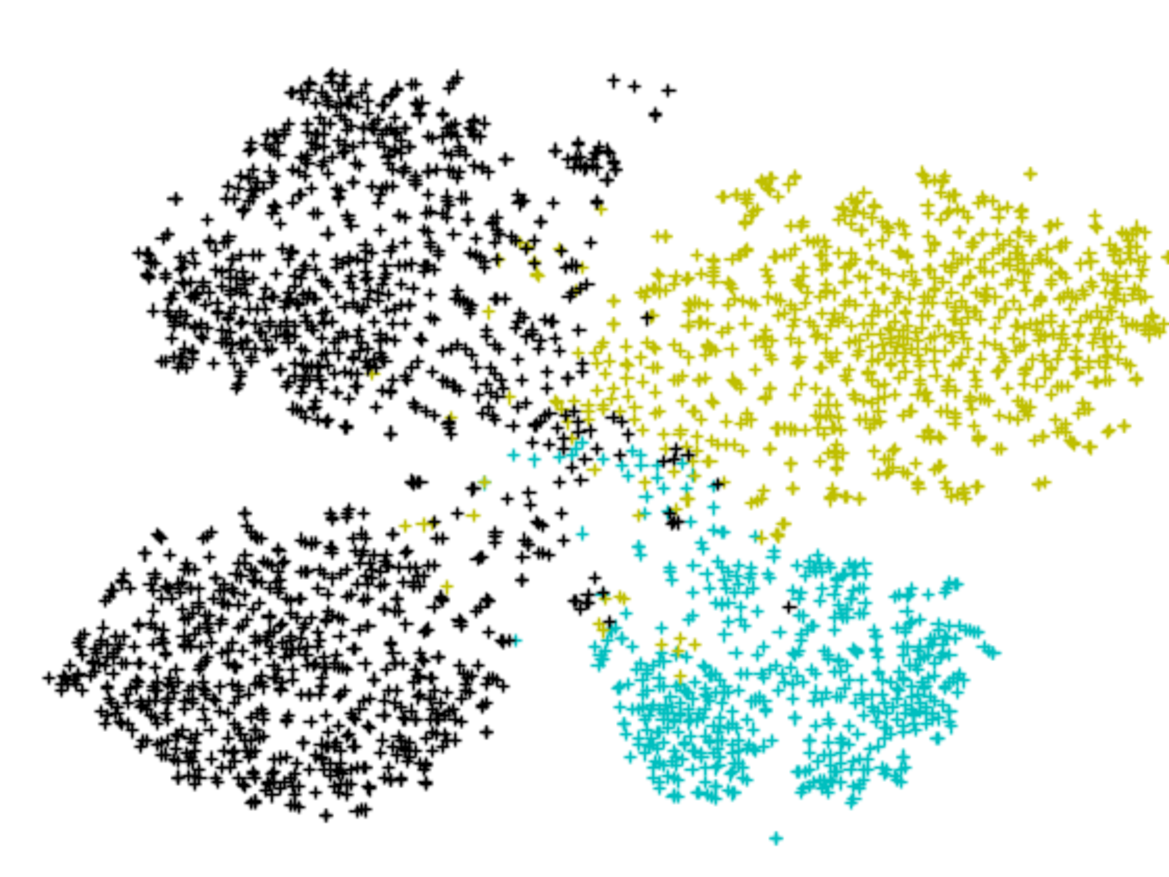
\includegraphics[width=\linewidth]{none}
    \caption{}
    \label{fig:null}
  \end{subfigure}
%
  \begin{subfigure}[b]{0.25\linewidth}
    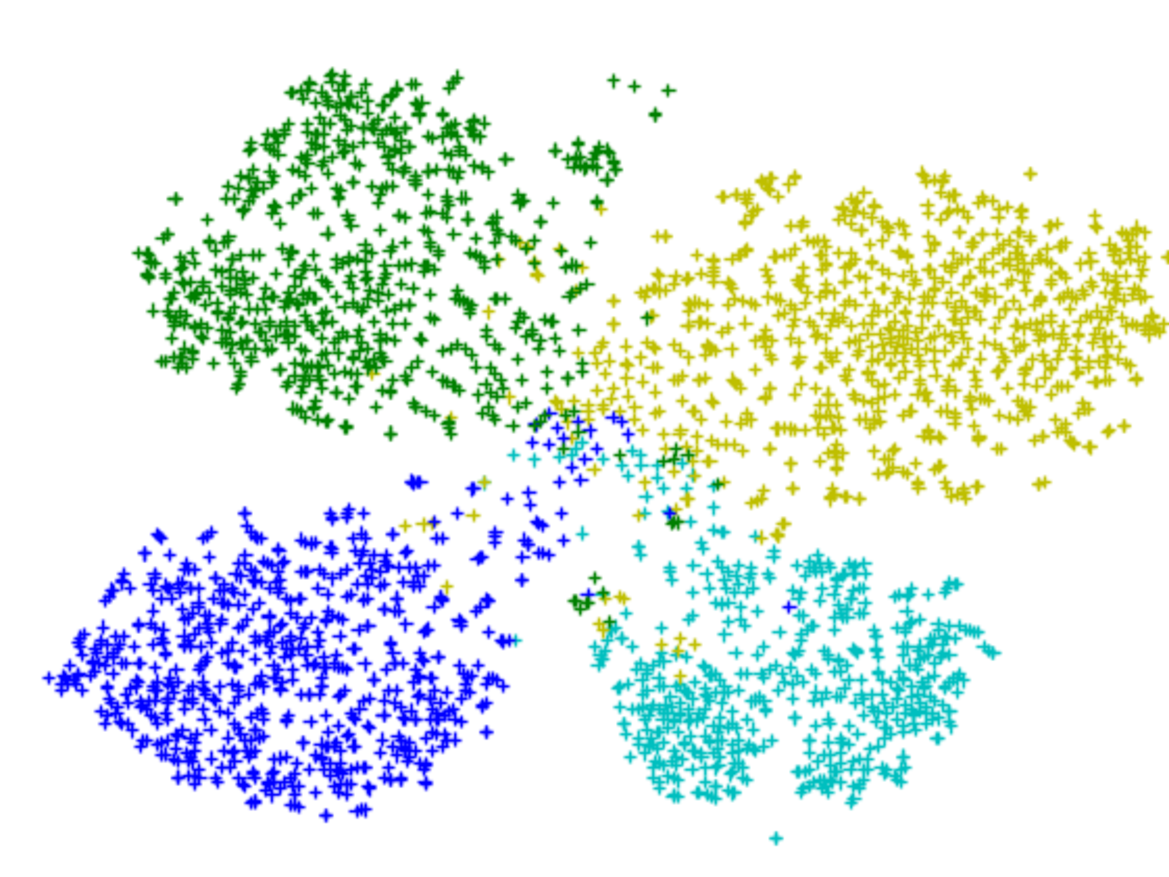
\includegraphics[width=\linewidth]{truth}
    \caption{}
% \caption{Points colored according to their ground truth labels}
    \label{fig:truth}
  \end{subfigure}
%
  \begin{subfigure}[b]{0.25\linewidth}
    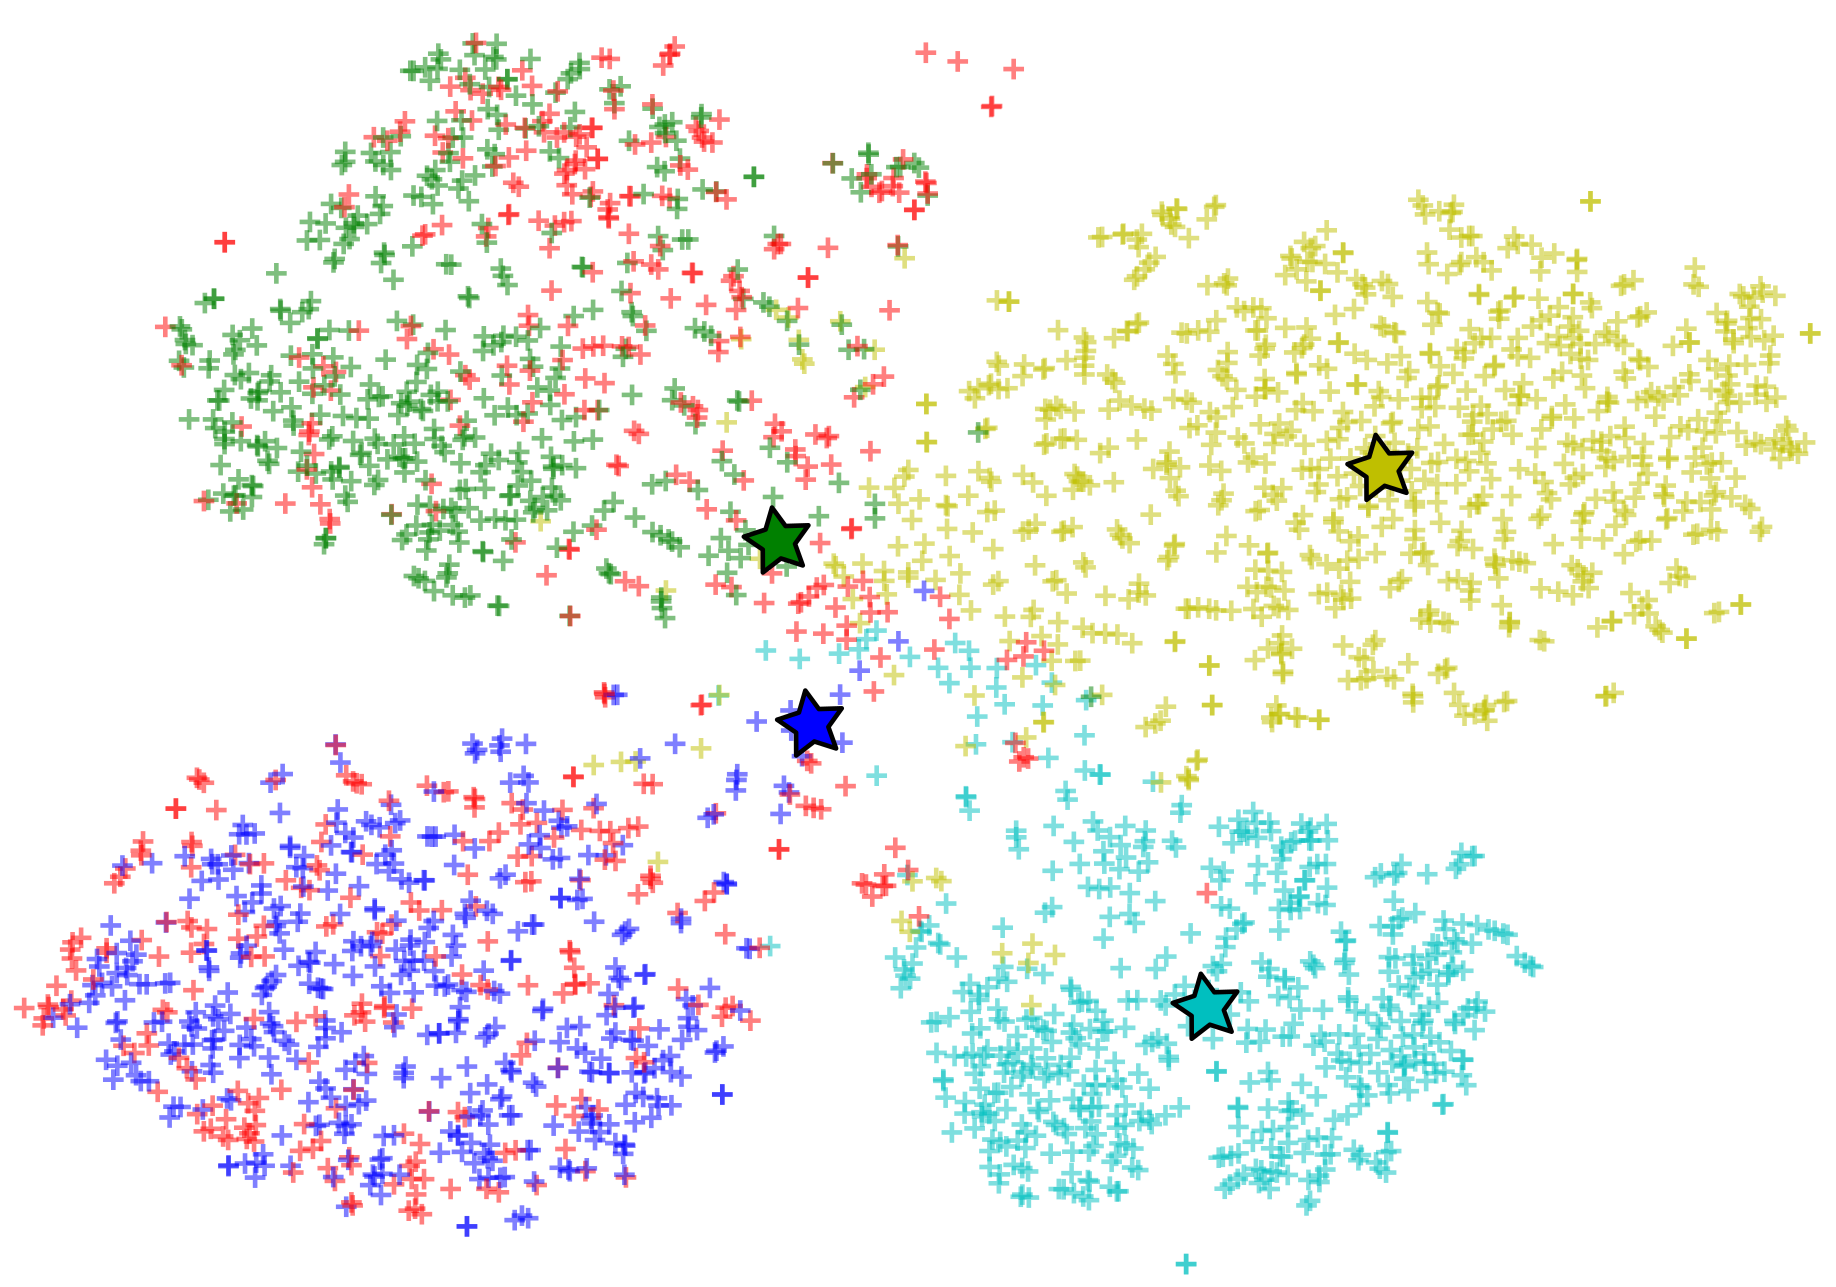
\includegraphics[width=\linewidth]{knn}
    % \caption{Signatures mapped to image spacing using Eq. \eqref{eq:dic} and denoted by stars. Then classification done using nearest neighbor}
    \caption{}
\label{fig:knn}
  \end{subfigure}
%
  \begin{subfigure}[b]{0.25\linewidth}
    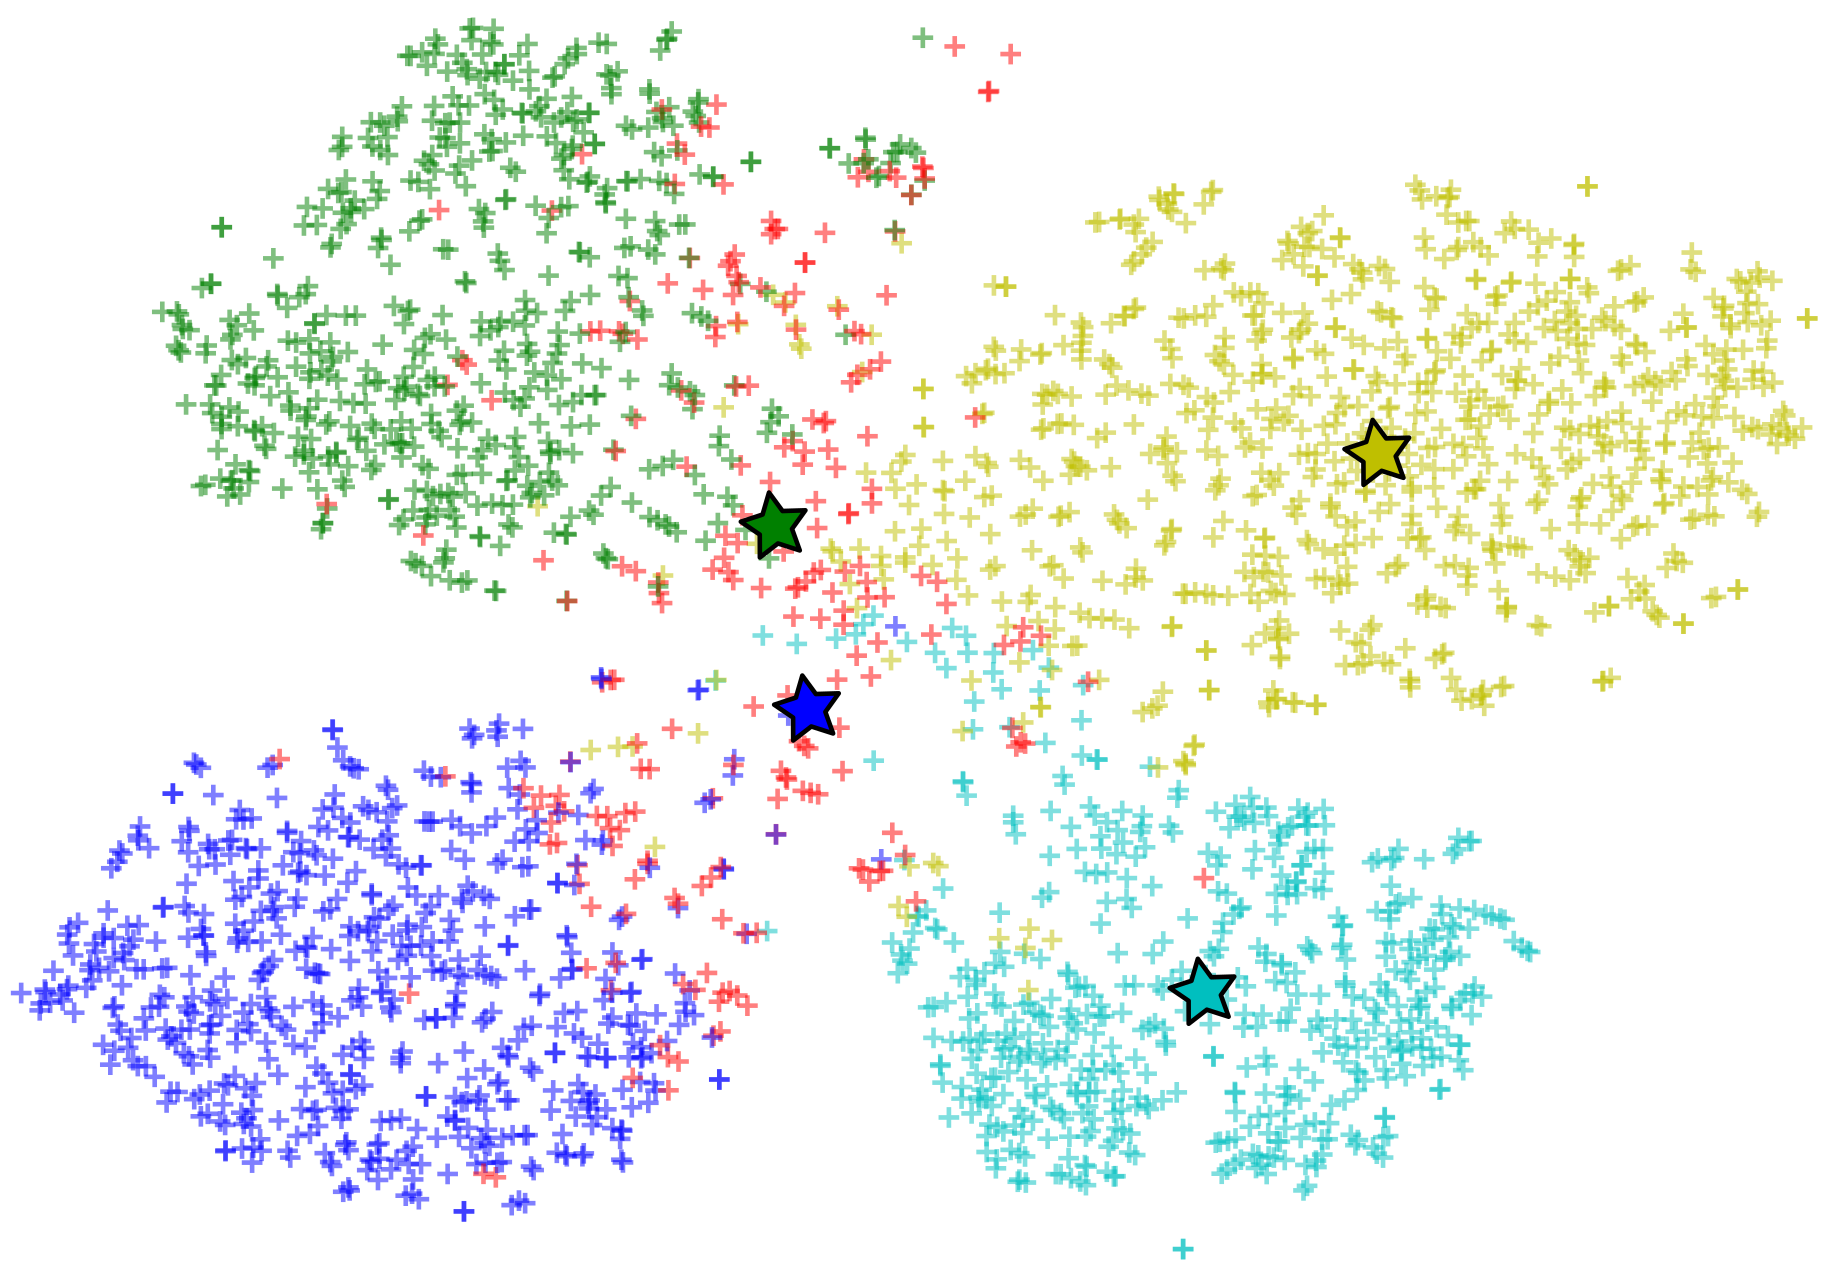
\includegraphics[width=\linewidth]{kmeans}
    % \caption{Stars as previous. Classification done by our compatibility function on cluster assignments from k-means}
    \caption{}
\label{fig:kmeans}
  \end{subfigure}
%
  \begin{subfigure}[b]{0.25\linewidth}
    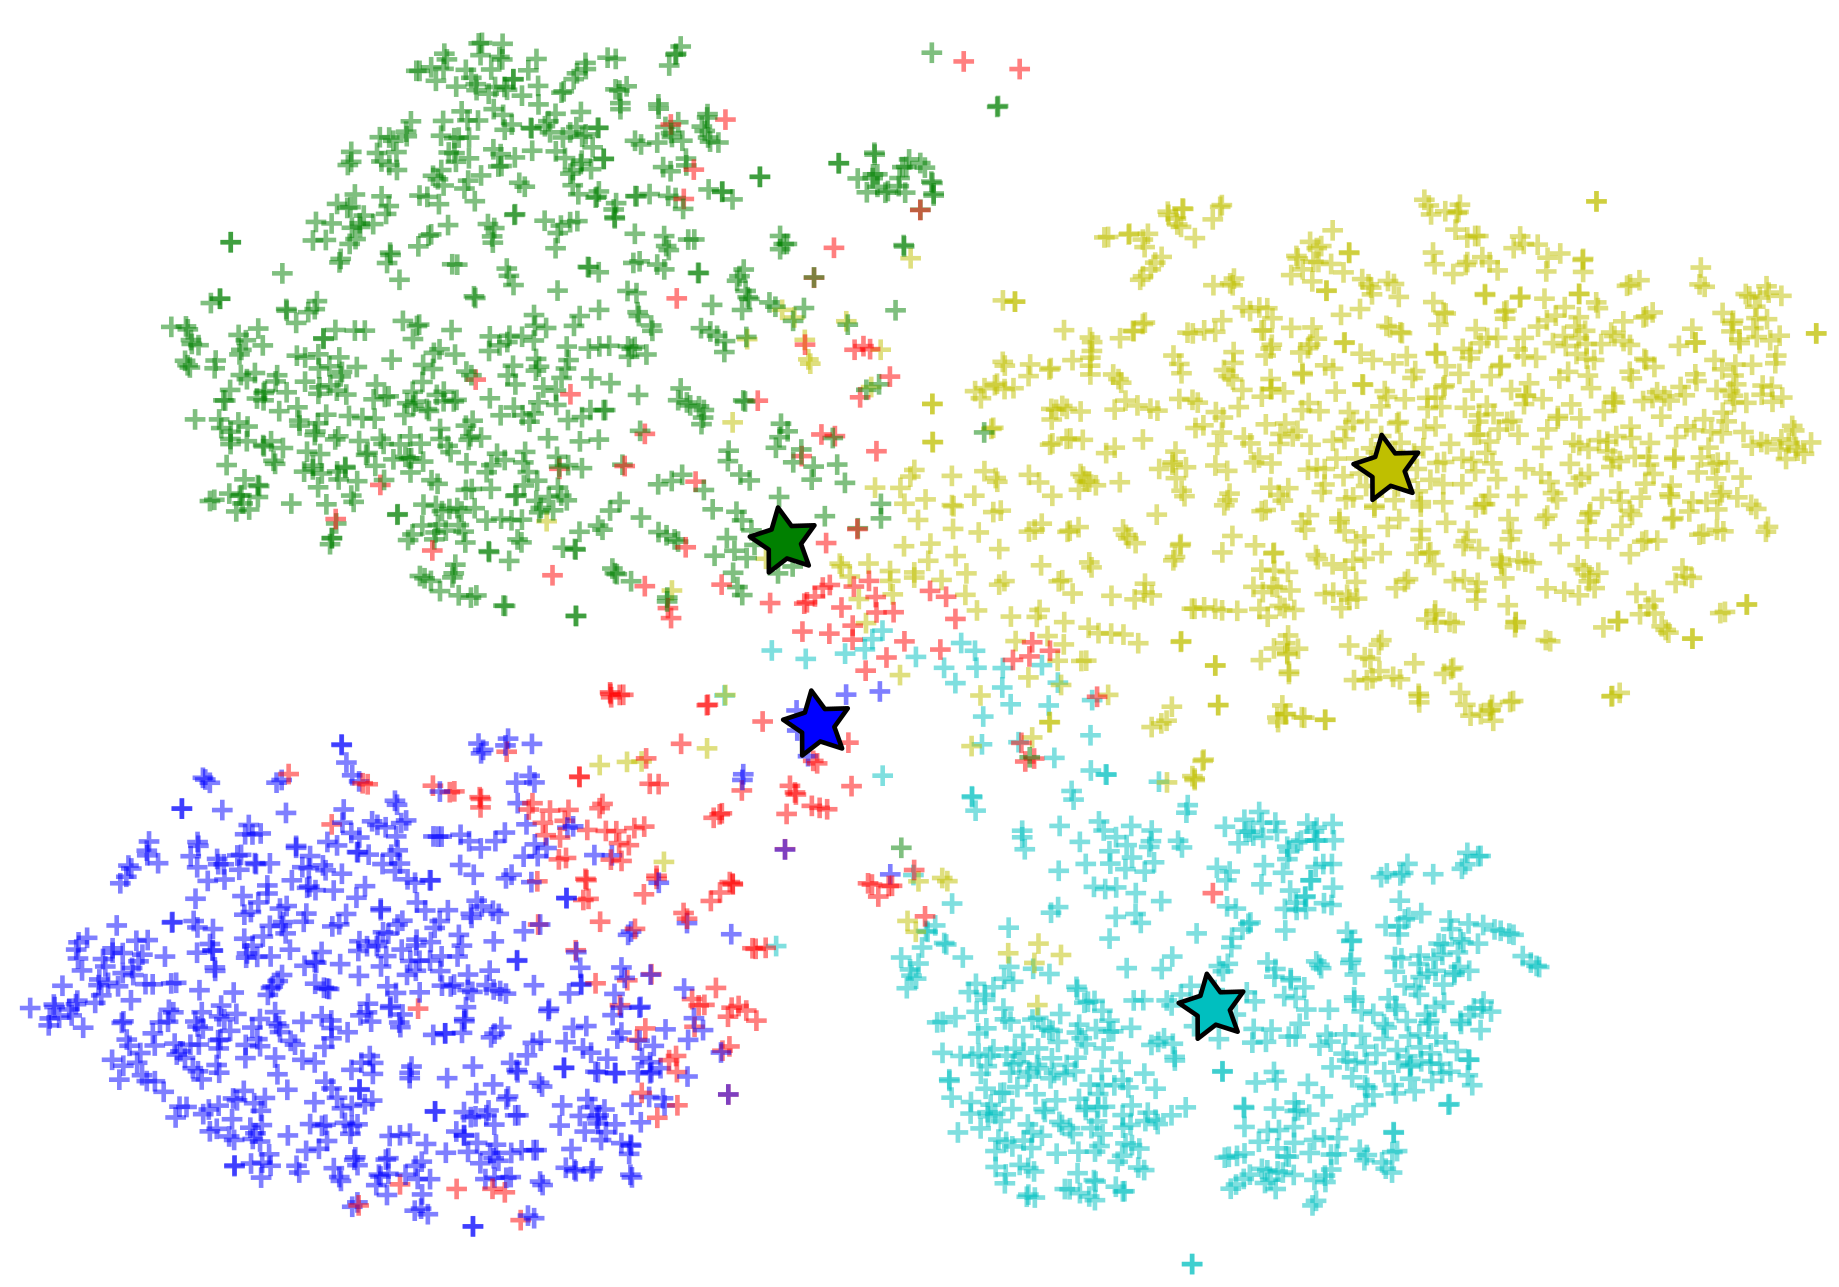
\includegraphics[width=\linewidth]{own_cluster}
    \caption{}
    \label{fig:clustering}
% \caption{Stars as previous. Classification by our compatibility function using our supervised clustering}
  \end{subfigure}
%
  \begin{subfigure}[b]{0.25\linewidth}
    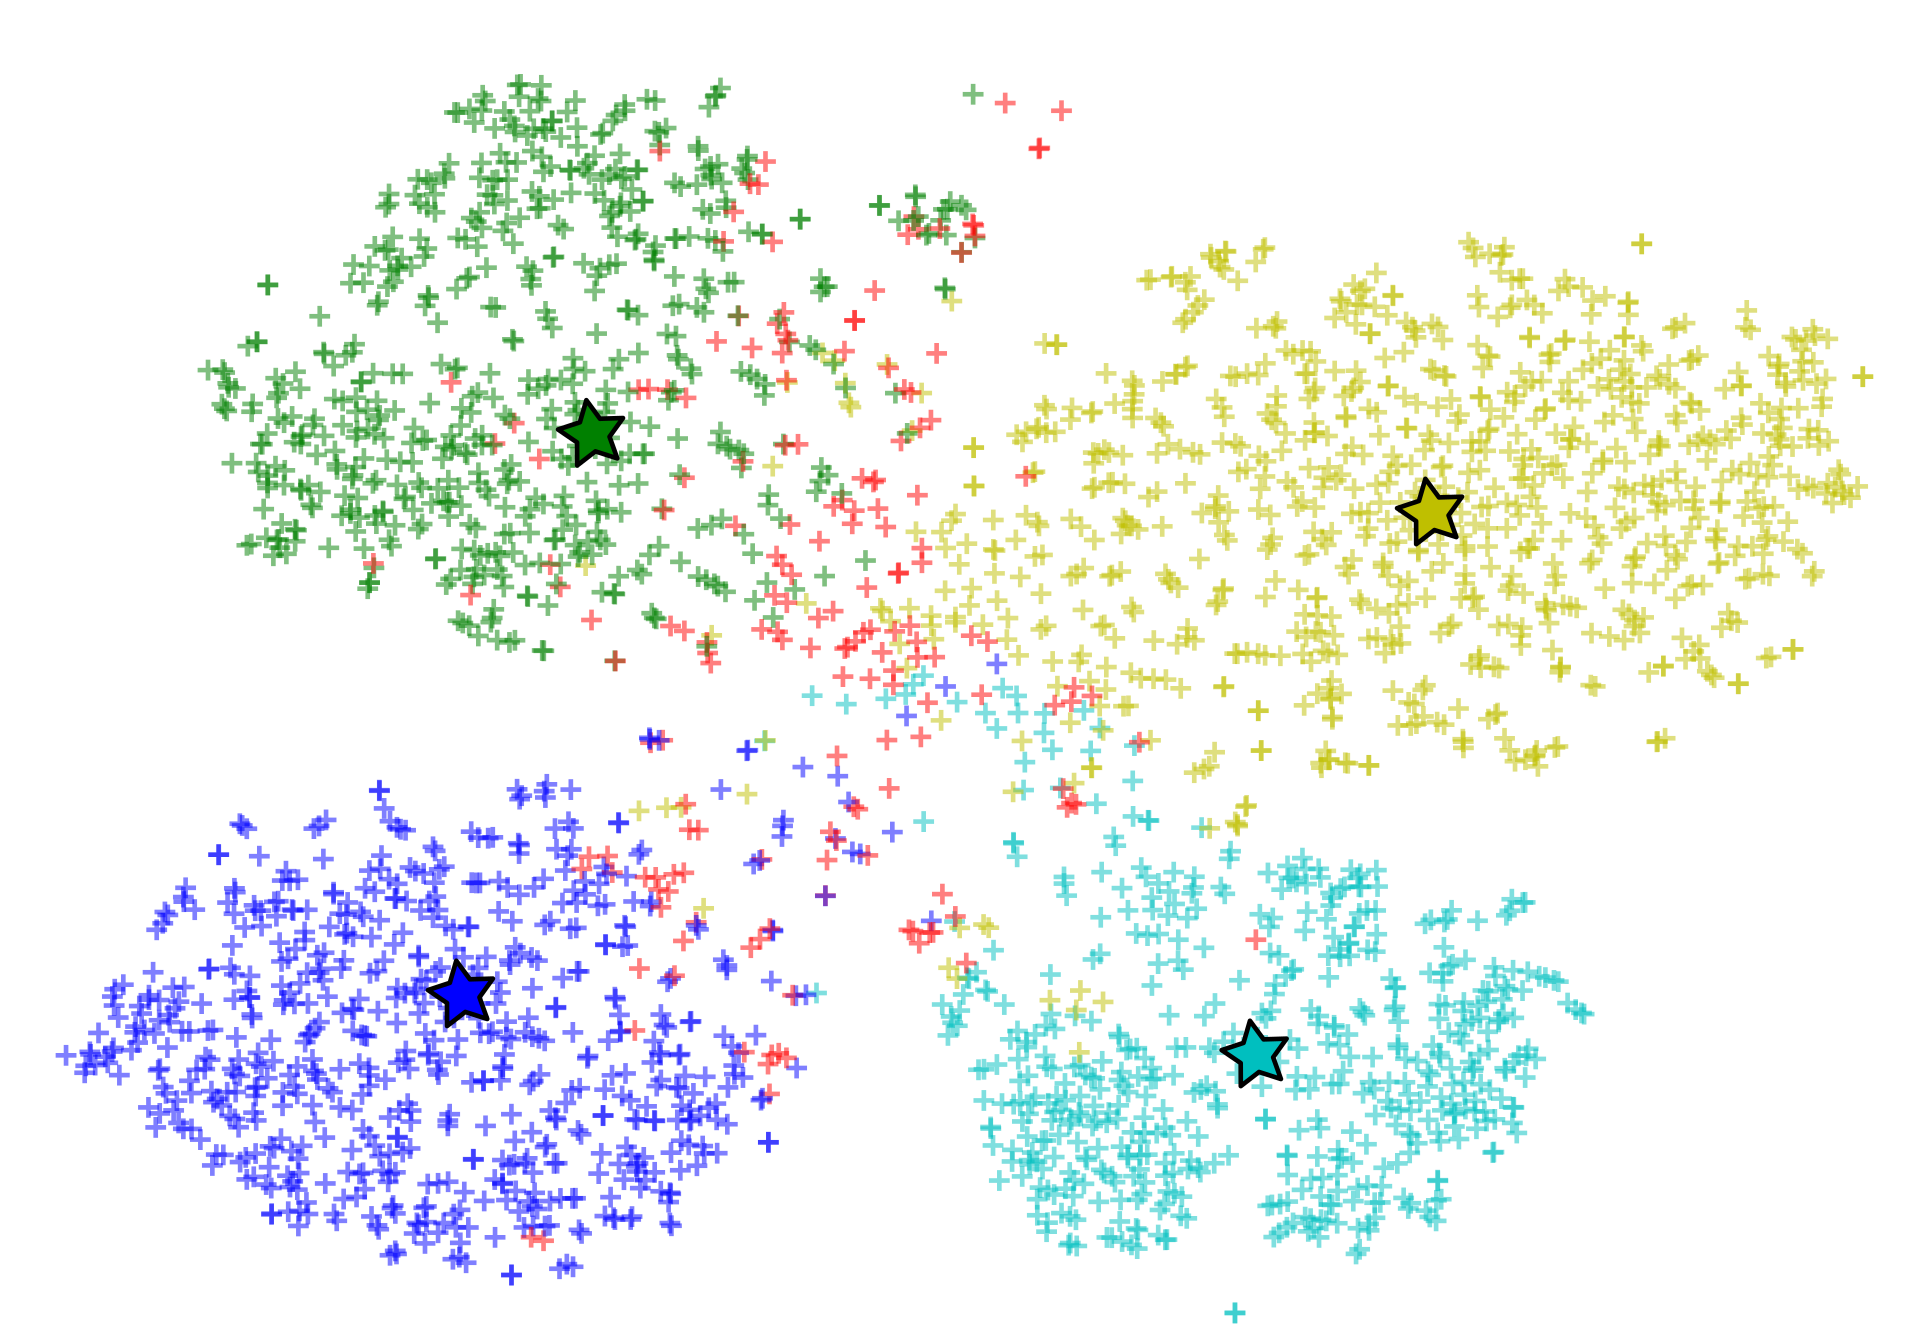
\includegraphics[width=\linewidth]{jeac}
    \caption{}
    \label{fig:joint}

% \caption{Class signatures mapped to image space (stars) and cluster assignment by JEaC}
  \end{subfigure}
  \caption{t-SNE embedding of the deep features for samples of four classes from AwA, two seen: antelope (cyan), grizzly bear (yellow) and two
  unseen: chimpanzee (blue), giant panda (green). Image samples are shown by plus signs and embedding of class signatures by stars.
  In Figs. c-f, red points denote assignment to a class other the four classes considered here. In Figs. c-e, the linear transformation in Eq. \eqref{eq:dic} is used to map signatures to the visual feature space.
  \textbf{a)} Data of seen classes are colored and those of unseen classes are black,
  \textbf{b)} Samples colored according to their ground truth labels,
  \textbf{c)} Classification by finding the nearest mapped signature,
  \textbf{d)} Classification done by our compatibility function on cluster assignments found by k-means,
  \textbf{e)} Classification by our compatibility function using our semi-supervised clustering,
  \textbf{f)} Cluster assignment and mapped signatures found by JEaC .
  }
  \label{fig:tsne}
\end{figure*}

% \textbf{Testing Cluster Assumption:}
% First, to give evidence for our key assumption of our method that instances from each class usually form a cluster in visual feature domains
% and to demonstrate effectiveness of our proposed clustering algorithm we design an
% experiment in which instances from unseen categories are clustered using our proposed clustering algorithm and also the k-means algorithm. Then,
% each cluster is assigned with a class label based on majority voting on ground truth labels. The number of clusters
%  is set to the number of classes as a natural choice.
%  \footnote{However we found out through experiment that increasing the number of clusters improves the accuracy.}
% For the k-means algorithm, we use the implementation available in Scikit-learn library \cite{scikit-learn} and run it with 20 different initializations
% and report results of that one with the best score.
% Accuracy of this labeling scheme that is based on clustering is reported in Table~\ref{tab:cluster}.
% These results shows the effectiveness of our proposed clustering method and that the cluster structure assumption in the visual semantic space is usually right.

\textbf{Cross Validation.}
To adjust parameters $\gamma$ and $\beta$ in Eq.~\eqref{eq:d_update} and parameter $\gamma$ in Eq. \eqref{eq:dic},
 training data are partitioned into train and validation sets.
We choose a number of categories randomly from training data as validation categories. For each dataset, the ratio of the categories in the
validation set to those in the whole train set is the sames as the ratio of the test categories to the total of the train and test ones.
In our experiments, we used $10-$fold cross validation, i.e. average results from ten different validation splits are used to decide on
optimal parameters.
Once optimal values for parameters are determined through the grid search by testing on validation set, the model
is then trained on all seen categories.

\subsection{Experimental Results}\label{results}
\textbf{Clustering experiment.}
First,  to  give  evidence  for  the  key  assumption  of  our method that samples of each class usually form
 a cluster in the space of deep visual features, we conduct an experiment in which samples of unseen categories
  (in the space of deep visual features) are clustered using a simple kmeans algorithm.
The number of clusters in this experiment is set to the number of unseen classes.
The kmeans implementation available in Scikit-learn library \cite{scikit-learn}
is used and the algorithm is run with 20 different initializations and the best score according
to the cost function of kmeans is selected. To evaluate clustering results,
the adjusted Rand Index is used and the obtained results are reported in Table \ref{tab:cluster}.
These results show that the cluster structure assumption in the deep visual space is valid to some extent and
thus we can use this assumption for the unsupervised task of labeling samples of unseen classes.


\textbf{Compared methods}
The proposed methods are compared with the most recent methods of zero-shot recognition shown in Table~\ref{tab:results}.
Among these methods, \cite{semi15,li15max} are semi-supervised zero-shot learning methods that use unlabeled samples of unseen classes during the training.
For other methods, we use the results reported in their original papers.
%Note that there may be some differences in experimental settings between some of other methods and ours.
Since we did not re-implement any of the other methods, if the original paper does not report results on a dataset we leave the corresponding cell as blank.

In Table~\ref{tab:results}, \textit{IEaC (K-means)} and \textit{IEaC (Proposed Clustering)} are the two versions of the IEaC method proposed
 in Section \ref{clustering}.
  In fact, \textit{IEaC (K-means)} uses the simple k-means clustering on samples
   of unseen classes and then utilizes Eq.~\ref{eq:label_assign} to assign labels to the clustered samples.
  However, \textit{IEaC (Proposed Clustering)} that has been shown in Algorithm~\ref{alg:ieac} performs
   the proposed semi-supervised clustering instead of the simple kmeans clustering. For our JEaC method,
 we introduced an iterative procedure in Section \ref{optimization} that starts by initializing $R$.
  Nonetheless, we can start by initializing either $W$ or $R$.
   \textit{JEaC(init W)} corresponds to initializing $W$ using Eq.~\eqref{eq:dic}
   and \textit{JEaC(init R)} denotes JEaC that initializes $R$ by the output of IEaC.
%
%    Moreover, if instance-level attribute vectors are available, true  attribute vector corresponding
%  to each labeled image can be used to construct $Y_s$ in \ref{eq:main} instead of the averaged class signature.
% \textit{JEaC(instance-attribute)} shows
%   results for such usage of attribute wectors in JEaC for three datasets that provide instance-level attribute vectors.

\textbf{Results.}
Results of the compared methods have been summarized in Table~\ref{tab:results}.
For our methods, the average and the standard deviation of different runs have been reported in Table~\ref{tab:results}. As it can be seen, the initialization of $R$ done by IEaC has an important role on the performance of JEaC. This can be justified by noting that the information about the distribution of
unlabeled data is leveraged when initializing $R$ (by the cluster assignment $R$ found in our IEaC method)
 while such information is absent in initializing $W$ as in Eq.~\ref{eq:dic}.
According to the results in Table~\ref{tab:results}, our JEaC (init R) method outperforms the other methods on all the four benchmarks. Although our IEaC method performs generally better than the existing zero-shot learning methods, our JEaC (init R) method outperforms IEaC too.

The effectiveness of different components of our methods is further illustrated in Figure~\ref{fig:tsne}. As it can be seen in
Figure~\ref{fig:knn} merely using mapping from Eq.~\eqref{eq:dic} results in poor signature embeddings and domain shift problem occurs. However, using the compatibility function proposed in Eq.~\ref{eq:label_assign} that is based on clustering of unseen data improves label assignments (Figure~\ref{fig:kmeans}) although there is no change in the mapped signatures.
Label assignments can also slightly be improved when the clustering method proposed in Section \ref{clustering} is used (Figure~\ref{fig:clustering}) instead of k-means (Figure~\ref{fig:kmeans}). Finally, as Figure~\ref{fig:joint} shows using
the mapping and class assignments found by JEaC, the domain shift problem is substantially alleviated and better signature embeddings are achieved.

\textbf{More Analysis.}
\begin{figure}[t]
  \centering
  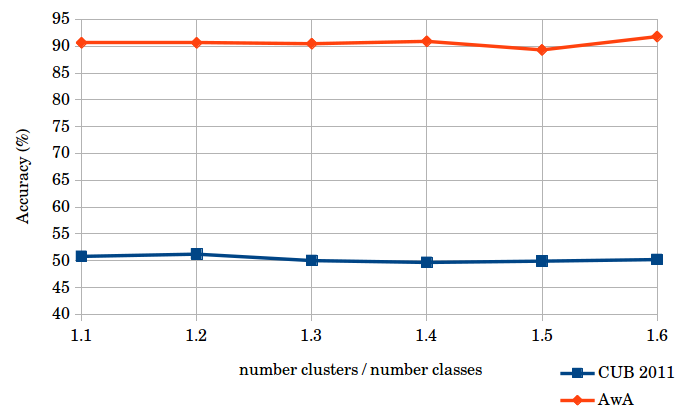
\includegraphics[width=\linewidth]{num_clusters}
  \caption{ Effect of number of clusters on multi class prediction accuracy for
  AwA and CUB 2011}
  \label{fig:n_culsters}
\end{figure}
\textcolor{red}{
We conduct more experiments to show that the performance of IEaC is not such sensitive to the number of clusters.
 In the aforementioned experiments, we had set the number of clusters to $n_s+2n_u$ for this method.
  However, according to Fig. \ref{fig:n_clusters}, we see that the IEaC performance is not such sensitive to the number of clusters and for a rather wide range of
   numbers results do not change significantly.
    Moreover, it is worth to mention that in our JEaC method number of clusters is no longer a parameter
     since we directly assign samples to the unseen classes in this method.
}
\begin{figure}[t]
  \centering
    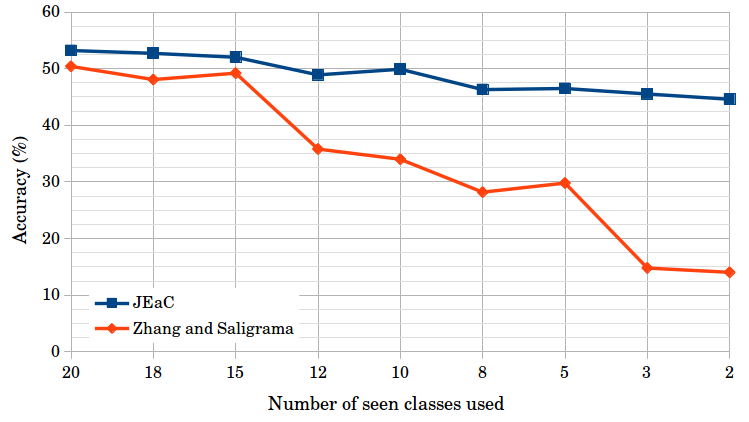
\includegraphics[width=\linewidth]{num_seen}
    \label{fig:n_seen}
    \caption{Comparing effect of number on seen classed used in training on zero-shot prediction accuracy
      in aPascal/aYahoo dataset between JEaC and Zhang and Saligrama \cite{agnostic}.
     }
\end{figure}

\textcolor{red}{
Since the performance of zero-shot classification methods depends on the number of seen classes,
 we intend to evaluate how much the performance of the proposed method degrades
  by decreasing the number of seen classes. We compare performance of our JEaC method and those of \cite{agnostic}
   (having highest accuracy among comparing methods in Table \ref{tab:results}) on aPascall/aYahoo dataset while fixing unseen categories
   and varying the number of seen categories used from the dataset.
  The results are presented in Fig. \ref{fig:n_seen} showing that JEaC is far less sensitive to number of seen categories and the gap between
  performance of JEaC and that of \cite{agnostic} widens when decreasing number of seen categories used in training.
  }


%
%
%
% We implemented our method using scikit-learn library \cite{scikit-learn} in Python.
% \footnote{Code is available at online :-?}
%  and used an Intel Core i5 CPU at 3.2 GHz to run the experiments.
%
\section{Conclusion} \label{conclusion}
In this paper, we proposed semi-supervised methods for zero-shot object recognition.
We used the space of deep visual features as a semantic visual space and learned a linear transformation to map class signatures to this
space such that the mapped signatures provide good representative of the corresponding instances.
We utilized this property that the rich deep visual features provide a representation space in which samples of each class
are usually condensed in a cluster. In the proposed method that jointly learns the mapping of class signatures and the class assignments of unlabeled data,
we used also unlabeled instances of unseen classes when learning the mapping to alleviate the domain shift problem.
Experimental results showed that the proposed method outperformed other recent methods with a large margin.
%\section*{Acknowledgement}

{\small
\bibliographystyle{ieee}
\bibliography{semi_zsl.bib}
}

\end{document}
